\documentclass{../template/tp}
\usepackage[utf8]{inputenc}
\usepackage{ucs}
\usepackage[frenchb]{babel}
\usepackage[T1]{fontenc}

\usepackage{graphicx}
\usepackage{amssymb}
\usepackage{amsmath}
\usepackage{wasysym} %smiley
\usepackage{hyperref}% hyperliens
\usepackage{tikz}
\usetikzlibrary{babel,positioning,calc}
\usepackage[]{circuitikz}
\usepackage{textcomp}
% \usepackage{minted}
\usepackage[long]{datetime}
\usepackage{gensymb} % \ohm, celsius
\usepackage{framed}
\usepackage{pdfpages}
\usepackage{mathastext} % math as standfard text : units are respecting typography conventions.
\usepackage{xspace} % typographie IN
\usepackage[all]{hypcap} %lien pointe en haut des figures
\langexam{frenchb}

\correction{false}
% \correction{true}

\author{The Fantastic Four}

\begin{document}

\tptitle{ELEC-H-301~: Électronique appliquée}{Séance 4~: les transistors MOS}

\section{Introduction}
\subsection{But}
Le but de ce TP est de vous rafraîchir la mémoire sur les transistors MOS.
\subsection{Prérequis}
Avoir lu le chapitre 17 du support de cours
\subsection{Objectifs}
À la fin de ce TP, vous devrez être capable :
\begin{itemize}
\item d'utiliser les notations des grandeurs liées au transistor MOS
\item de comprendre la polarisation du transistor MOS et ses conséquences sur le point de fonctionnement
\item de réaliser un schéma à petit signal d'un montage à transistor
\item d'extraire les paramètres intéressant de la documentation d'un transistor en vue de dimensionner un étage.
\item d'aborder sereinement des exercices de dimensionnement et le laboratoire portant sur le transistor MOS.
\end{itemize}
\subsection{Lexique}
%\section{Get ready, Set! Go!!!!}
\newpage
\section{Notations}
L’objectif de cette question est de vous familiariser avec les notations des différentes grandeurs électriques liées à l'utilisation d'un transistor MOS.

Soit le schéma électrique du transistor MOS et son équivalent à petit signal~:

\begin{center}
%\shorthandoff{:!}
		\begin{circuitikz} \draw
		(2.25, 1) node[nfet] (mos) {}
%		(0,0) -- (2,2)
%		(0,0) node[nfet]{} -- (2,2)
		%(mos.B) node[anchor=west] {B}
		%(mos.G) node[anchor=east] {}		
		(mos.D) -- (2.25, 2) to  [short, -o](3.25, 2)  node[anchor=west] {D}		
		(mos.S) -- (2.25, 0) to [short, -o](3.25, 0)  node[anchor=west] {S}		
		(mos.B) -- (mos.S)
		(2.25,0) to [short, -o](0,0)  node[anchor=east] {S}		
		(0,2)  node[anchor=east]{G}[short, o-] to  (1,2) 
		(1,2) -- (1,1) -- (mos.G)
		%(gin) -- (mos.G)
		;\end{circuitikz}\hspace*{1cm}
		\begin{circuitikz}\draw
		(0,0) node[anchor=east] {g} 
		to [short, o-] (1,0) 
		to [open, v={~}] (1,-2)
		to [short, -o] (4,-2)
		to  (0,-2) node[anchor=east] {s}
		%to [short] (3,-2)
		(3,0) to [cI, i={~}] (3,-2)
		(3,-2) to [short, -o] (4,-2) node[anchor=west] {s}
		(3,0) to [short, -o] (4,0)
		to node[anchor=west] {d} (4,0)
	;\end{circuitikz}
%\shorthandon{:!}		
	\end{center}

	%\vspace*{-0.5cm}
\Question{~\\%~\\ %sinon, ça fait dlm
Remplir le tableau suivant et indiquer les grandeurs sur le schéma.\vspace{-1.5Em}
\center
\begin{tabular}{|c|c|c|c|c|}
\hline 
{grandeur} &{\hspace*{1cm}nom\hspace*{1cm}} &{\hspace*{2cm}signification\hspace*{2cm}} & {statique} & {dynamique}\\ 
\hline 
$V_{GS}$ &  &  &  &  \\ 
\hline
$v_{gs}$ &  &  &  &  \\ 
\hline
$V_{DS}$ &  &  &  &  \\ 
\hline
$v_{ds}$ &  &  &  &  \\ 
\hline
$I_{D}$ &  &  &  &  \\ 
\hline 
$g_{m}$ &  &  &  &  \\ 
\hline 
$g_{m}\cdot v_{gs}$ &  &  &  &  \\ 
\hline 

\end{tabular} 

	
	
	
}%
{
	bar
}
\newpage
\section{Amplifier avec une source de courant commandée idéale (10 minutes) }
Afin de réaliser un amplificateur \textbf{tension--tension}, on se propose d'utiliser un transistor MOS. 
%
Or le transistor MOS se comporte comme une source de \textbf{courant} -- non idéale -- commandée en tension. % et ne peut donc pas être utilisé immédiatement pour réaliser une source de tension commandée en tension.
%
%L'intérêt du transistor MOS est de se comporter comme une source de \textbf{courant} commandée en tension, malheureusement imparfaite. %Dans un premier temps, considérons une source idéale.
%
%Voyons d'abord comment construire un amplificateur tension--tension en utilisant une source de courant commandée en tension \textit{idéale}.
%
%La première étape sera d'amplifier de tension à tension en utilisant une source de courant \textit{idéale} commandée en tension.
%
La source \textit{idéale} utilisée est représentée figure \ref{fig:source}\footnote{NB : le symbole européen de la source de courant commandée est utilisé ici}.
%
\begin{figure}[h!]
	\begin{center}
		\begin{circuitikz}\draw
			(0,0) node[anchor=east] {s} 
			to [short, o-] (1,0) 
			to [open, v=$v_{gs}$] (1,-2)
			to [short, -o] (0,-2)
			to  (0,-2) node[anchor=east] {s}
			%to [short] (3,-2)
			(3,0) to [cI=$ g \cdot v_{gs}$] (3,-2)
			(3,-2) to [short, -o] (4,-2) node[anchor=west] {s}
			(3,0) to [short, -o] (4,0)
			to node[anchor=west] {d} (4,0)
		;\end{circuitikz}
	\end{center}
\caption{Source de courant commandée en tension}
\label{fig:source}
\end{figure}


%\subsection{Caractéristique de transfert de cette source commandée idéale}
%équations + courbes ??

Cette source \textit{idéale} absorbe un courant proportionnel à la tension d'entrée selon la~loi : $$i_d = g \cdot v_{gs}$$

où $g$ est la transconductance de la source. 


\Question{
\begin{itemize}
\item À quelle condition cette source est-elle linéaire ?
\item Tracer sa caractéristique de sortie.
\item Que faut-il ajouter pour obtenir un amplificateur tension--tension.
\end{itemize}
	
	\label{Q:1}
	
	}
	{$g$ doit être constant.}
	
	\newpage
\section{Polarisation et point de fonctionnement}
Rappel TP3 : résoudre ce circuit à AOP avec polarisation :


\Question{
Soit le circuit suivant, calculer les tensions et courants \textbf{continus} en tout point du circuit.
\begin{center}
			%\includegraphics[width=8cm]{}
			\begin{circuitikz}[scale=1]\draw
			(0,1) to [short,o-] (9,1)
			(4,6) to [short] (9,6)
			(0,3) node[anchor=east] {In} to [short,o-] (1,3)
			(0,3) to [open, v_=$V_{in}$]  (0,1)
			(1,3) to [C=$C_{in}$ ](1.5,3)
			(1.5,3) to [short,-*] (2,3)
	%
			(2,6) node[anchor=south ] (alim) {$+V_{DC}$}
			(1.6,6) -- (2.4,6) %bar under the label
			%(alim.text) node {}
	%		
			(2,3) to [R, l_=$R_{B1}$](2,6)
			(2,3) to [R=$R_{B2}$](2,1)
	%		
			(4,3) node[nfet] (mos) {}
			%(mos.B) node[anchor=west] {B}
			(mos.G) to [short] (2,3)
	%		
			(mos.D) to (4,4) to [R, l_=$R_D$] (4, 6)		
			%(4,5.5) to [R] (mos.D)
	%		
			(mos.D) to [short,-*](4,3.5)  to [short] (4.25,3.5)
	%		
			(mos.S) to [short] (4,1)% to [short, -o](2,0)  node[anchor=west] {S}
			(mos.S) -- (mos.B) %source to bulk connection		
	
			(4.25,3.5) to [C, l^=$C{out}$] (6,3.5) to  [short](6,3.5) to [short,-o](6.5,3.5)node [anchor=south] {Out}	
			(6,3.5) to [generic, l_=$Z_{ch}$] (6,1)
			(6.5,3.5) to [open,v^=$V_{out}$] (6.5,1)
	%		
			(9,1) to [battery, l_=$E$](9,6)
	%		%(1,0) to [short, -o](-1,0)  node[anchor=east] {S}
	%		
	%%			(0,0) node[anchor=east] {In} 
	%%			to [short, o-] (1,0) 
	%%			to [open, v=$V_{GS}$] (1,-2)
	%%			to [short, -o] (0,-2)
	%%			to  (0,-2) node[anchor=east] {S}
	%%			to [short] (3,-2)
	%%			(3,0) to [cI=$ g_m \cdot V_{GS}$] (3,-2)
	%%			(3,-2) to [short, -o] (4,-2) node[anchor=west] {S}
	%%			(3,0) to [short, -o] (4,0)
	%%			to node[anchor=west] {D} (4,0)
	%	%		
			;\end{circuitikz}
	\end{center}
	
	Valeurs des composants/sources : 	
	
	Placer le point de fonctionnement sur les courbes caractéristiques du BS170 en annexe.
	
	}
	{%
	}

%TODO : ajouter droite de charge
%TODO : qqch fait dlm avec l'espace avant itemize

\section{Schéma à petit signal}

\Question
{
%question
Sachant que $V_{DC}$ a été judicieusement choisie de manière à obtenir $g_m=0.1S$, déterminer le schéma à petit signal du montage présenté à la question précédente.
 
 \begin{itemize}
 \item Calculer le gain du montage. Les condensateurs peuvent être assimilés à des court-circuits dans la bande passante du montage.
 \item Calculer les impédances d'entrée et de sortie du montage.
 \item Calculer la fréquence de coupure à l'entrée et à la sortie du montage (\textit{i.e.} l'approximation du premier point n'est plus valable).
 \item Bonus : donner l'expression des impédances d'entrée et de sortie ainsi que le gain pour toute fréquence. Quel est le comportement de ce montage ?
 \end{itemize}

}
{%answer
}



\section{Lecture de documentation~: extraction de paramètres}

Sachant que $ID=42mA$, déterminer le $V_{GS}$ et le $g_m$ correspondant sur base des courbes en annexe.

\section{Exercices}
Sur base des courbes disponibles en annexe, dimensionner un étage à transistor MOS de gain -18.973 pour chacun des transistors. 

\section{Exercice d'examen}

\Question{
	foo
}%
{
	bar
}
\appendix
\section{Caractéristiques}
%\subsection{BS170}
\subsection{Caractéristiques du transistor NMOS BS170}
%\vspace{1cm}
\label{anx:mos_doc}
\begin{center}
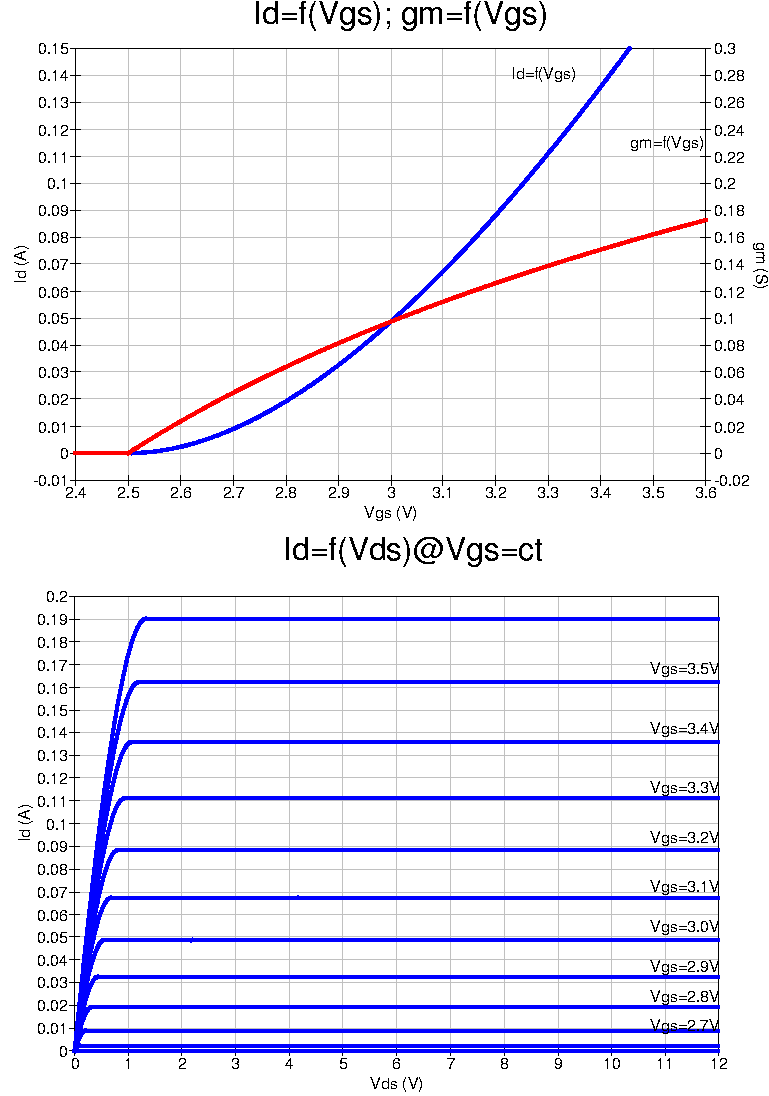
\includegraphics[width=16cm]{bs170_courbes_2k14_ok-crop.pdf}
% TODO : enlever le n° de page
% les courbes ici sont ont été corrigée et sont cohérentes.
\end{center}

%\addcontentslinenono{toc}{section}{\href{http://pdf.datasheetcatalog.com/datasheets/70/123316_DS.pdf)}{\numberline{B}Documentation du transistor NMOS (lien cliquable)}}
%{\href{http://pdf.datasheetcatalog.com/datasheets/70/123316_DS.pdf}{\attachfile[icon=Graph, color=0 0.75 1,description =Documentation du transistor NMOS BS 170 ]{./Documentation_BS170.pdf}}}

\subsection{IRF150/BUZ11???}

% TODO : fancy header
\end{document}
